\documentclass[11pt]{article}
\usepackage[margin=1in]{geometry}
\usepackage{amsmath,amssymb,booktabs,graphicx,array,tabularx,hyperref}
\usepackage[T1]{fontenc}
\usepackage{lmodern}
\usepackage{natbib}
\title{Conditional Prospective Deliberation in Heterogeneous Learning Teams:\\Performance--Computation Trade-offs and Generalization Limits}
\author{Author information withheld for scientific review}
\date{Draft: 12 October 2026}
\begin{document}
\maketitle
\begin{abstract}
Allocating prospective decision computation selectively may reduce deliberation cost, but learned routing rules can alter the future states on which their own decisions depend. We characterize this trade-off in a controlled sequential simulator of three-agent teams with heterogeneous, experience-dependent capabilities and Bayesian uncertainty about task requirements. A fast operator maximizes immediate belief-expected production; a deep operator additionally anticipates the consequences of actions for future observations and capability development. A frozen Ridge predictor routes between these operators using ex-ante capabilities, beliefs, and remaining time, with a cost-normalized proxy for prospective production advantage. We evaluate this state-informed policy against independent random invocation and constant fast/deep baselines on 868 paired histories across four crossed team-geometry and environment partitions. Under an equally weighted four-domain estimand, the selected 50\% routing point improves cumulative latent production relative to random routing by 0.1167 (95\% paired bootstrap interval [0.0310, 0.2013]) while reducing measured decision computation by 0.1924 seconds per history (interval [-0.3539, -0.0228]). The production difference is approximately 0.22\% of the random baseline. Positive production contrasts are supported for development-team geometries, but not for held-out team geometries. The actual invocation frequencies differ, so the comparison does not establish efficiency at exactly equal compute budgets. The study provides a bounded empirical characterization of conditional deliberation and its generalization limitations, not a new metareasoning theory or an optimal value-of-computation estimator.
\end{abstract}
\section{Introduction}
Sequential agents face a choice not only among physical actions but also among computational procedures used to select them. Prospective planning can account for the effects of a current action on future information and future productive capabilities; it also incurs computational cost. In systems where decisions change the capabilities available later, a learned rule for invoking planning can induce its own future state distribution. This creates a setting in which a supervised advantage proxy may be useful locally without transferring reliably to other initial capability configurations.

This paper reports a frozen, controlled experimental characterization of conditional deliberation in a heterogeneous learning system (HLS), where physical decisions change persistent capabilities and thereby affect later states and routing opportunities. Its contribution is empirical, not algorithmic: (i) a reproducible comparison of one state-informed routing rule with independent random invocation and constant FAST/DEEP references; (ii) paired evaluation across crossed development/held-out team and generator-kernel partitions; and (iii) explicit documentation of the small aggregate gain, unequal realized invocation frequencies, and the failure to establish a production advantage on held-out team geometries. The feedback of interest is deliberation selection -> assignments and exposure -> capability evolution and policy-dependent visited states -> subsequent deliberation selection. We make no claim of superiority over informed routing alternatives, which were not evaluated.

\section{Related work}
Rational metareasoning treats computation as a decision whose expected consequences depend on subsequent physical action \citep{russell1991,hay2012}. The algorithm-selection problem formalizes choosing among procedures from instance characteristics \citep{rice1976}; SATzilla is a learned portfolio example \citep{xu2008}; and adaptive computation time varies computational effort with input-dependent processing in recurrent networks \citep{graves2016}. These works establish the general ideas of computation allocation, learned selection, and adaptive effort; none is claimed as novel here. FAST/DEEP selection, supervised routing, an estimated deliberation benefit, computational costs, and a benefit-per-cost score are all design elements of this evaluated prototype, not claimed algorithmic contributions. The empirical focus is narrower: how one fixed routing rule behaves when its physical actions alter persistent capabilities and hence the states encountered by later decisions.

The deep operator is related to Bayesian planning and dual control, in which decisions influence both future states and information \citep{klenske2016}. Learning and exploitation can create long-run trade-offs in adaptive systems \citep{march1991}. Finally, policy-dependent state distributions are a recognized concern in sequential learning \citep{ross2011}. The present work does not establish a new distribution-shift mechanism or a causal explanation of geometry effects; it measures a particular routing comparison under explicitly partitioned synthetic conditions.

\section{HLS environment and mathematical model}
Let $S=(s_{ik})\in[0,1]^{3\times2}$ denote the capability matrix of three agents for two dimensions. At each decision, $X=(x_{ik})$ is selected from a fixed enumerated set $\mathcal A$ of 64 assignments, subject to $\sum_k x_{ik}\leq1$. Aggregate output is $Y_k(S,X)=\sum_i x_{ik}s_{ik}$. For requirement weights $z=(p,1-p)$, latent physical production is
\begin{equation}
R_z(S,X)=\left(\sum_{k=1}^2 z_k Y_k(S,X)^\rho\right)^{1/\rho},\qquad \rho=0.5.
\end{equation}
The external outcome $\mu_{\mathrm{true}}$ is the sum of this latent production across decisions, not the sum of noisy observations. The agent does not know the true current requirement vector and maintains a finite Bayesian belief $b=(b_1,b_2,b_3)$ over $\hat z_1=(0.8,0.2)$, $\hat z_2=(0.5,0.5)$, and $\hat z_3=(0.2,0.8)$. Observations have a Gaussian likelihood with standard deviation $\sigma=0.10$. We denote the posterior given prospective observation $r$ by $B(b,S,X,r)$.

Capabilities change with experience according to the frozen MIS-v2 transition
\begin{equation}
F(S,X)_{ik}=1-(1-s_{ik})\exp(-\lambda x_{ik}),\quad
\lambda=-\log(1-\eta),\quad\eta=0.35.
\end{equation}
Thus capability development persists across problems, whereas beliefs reset to the uniform prior at each problem boundary. Each history comprises 12 problems with three decisions each (36 decisions), generated by a frozen STAY/MOVE/RETURN environmental kernel. The physical generator family is a synthetic experimental subset, not a model calibrated to observed teams. In particular, for fixed cumulative exposure the terminal capability under this transition depends on total exposure rather than its ordering; path effects in the experiment arise through intermediate rewards, decisions, and policy-induced exposures.

\section{Conditional prospective deliberation}
\subsection{FAST and DEEP}
The immediate internal objective is
\begin{equation}
g(b,S,X)=\sum_{m=1}^3 b_m R_{\hat z_m}(S,X).
\end{equation}
FAST chooses $X_F\in\arg\max_{X\in\mathcal A}g(b,S,X)$, using the frozen enumeration and $10^{-10}$ tie tolerance. It is action-equivalent to the existing Q00 operator because the Q00 continuation term is independent of the candidate current action. It avoids posterior branching, capability forecasting, and future action searches.

At a nonterminal decision, DEEP is the frozen Q11 information-and-development operator:
\begin{equation}
Q_{11}(b,S,X)=g(b,S,X)+\sum_{m=1}^3 b_m\sum_{j=1}^3\omega_j\max_{U\in\mathcal A}g\!\left(B(b,S,X,r_{mj}),F(S,X),U\right).
\end{equation}
Here $(r_{mj},\omega_j)$ are the frozen three-node Gauss--Hermite observation quadrature and weights; posterior likelihoods use the pre-development state $S$. DEEP chooses the action maximizing $Q_{11}$ with the same tie convention. The effective planning windows within each three-decision problem are 2, 2, and 1; planning does not cross problem boundaries. At terminal decisions all policies use FAST.

\subsection{Supervised routing rule}
The frozen standardized Ridge model uses ten ex-ante features: the six capability entries, three belief probabilities, and normalized clock $\tau/36$. Its regularization parameter is $\alpha=10$. The supervised target is a Monte Carlo production difference between Q11 and Q00 under fixed Q11 continuation. It is \emph{not} the recursively adaptive value of invoking DEEP now and then following the META routing policy. Moreover, production and computation seconds are not converted to a common utility.

For nonterminal states, the META-VOC routing score is
\begin{equation}
q(S,b,\tau)=\frac{\max\{0,\widehat{\Delta R}_{\mathrm{Ridge}}(S,b,\tau)\}}{\widehat{\Delta t}(h)},
\end{equation}
where $h$ is the number of remaining within-problem decisions. Frozen incremental costs are $\widehat{\Delta t}(2)=0.209201959$ s and $\widehat{\Delta t}(3)=0.209788291$ s. Because these denominators are nearly equal, the score primarily ranks predicted production advantage; it is not a state-dependent computational cost model. Three thresholds calibrated once on 1,400 validation states yield nominal routing points 25\%, 50\%, and 75\%: 0.2291733537, 0.1670898304, and 0.1108507124, respectively. The implementation also preserves frozen feature-hash tie cutoffs. Above threshold, META invokes DEEP; otherwise it executes FAST without evaluating DEEP. The earlier ungated META prototype invoked DEEP in 97.07\% of eligible decisions, a negative result motivating explicit routing calibration.

\section{Experimental methodology}
The development-stage comparison used 420 histories from 20 development teams and 21 development kernels, with retrospective exact matching of RANDOM's DEEP invocation count. Development paired production differences for META minus RANDOM at 25\%, 50\%, and 75\% were respectively $0.1281$ (95\% interval $[-0.0522,0.2979]$), $0.2337$ ($[0.1030,0.3686]$), and $0.1163$ ($[0.0090,0.2307]$). These results motivated selecting 50\% as primary. Consequently, the primary operating point was \emph{not} selected independently of development data, although all confirmatory histories and analysis procedures were frozen before confirmatory execution.

The confirmatory design crossed 20 development versus eight held-out teams with 21 development versus ten held-out kernels (Table~\ref{tab:domains}). There was one new independent exogenous history per team--kernel cell: 868 histories, eight policies, 6,944 trajectories, and 249,984 decision records. Within each matched history, all policies shared physical problem sequences and standard-normal observation innovations, but generated their own observations, beliefs, capabilities, assignments, and visited states. Thus pairing controls exogenous histories but does not make endogenous states identical across policies. Confirmatory RANDOM used independent frozen Bernoulli invocation priorities at nominal probabilities 0.25, 0.50, and 0.75; it was not retrospectively call-count matched.

\begin{table}[ht]\centering\small\caption{Frozen confirmatory generalization partitions. These are separate claims about fresh histories, generator kernels, and team geometries, not a decomposition of their causal effects.}\label{tab:domains}\begin{tabularx}{\linewidth}{l l l X r}\toprule Domain & Team partition & Kernel partition & Interpretation & Histories\\\midrule G1 & Development & Development & Fresh histories from represented teams/kernels & 420\\ G2 & Development & Held-out & Compositional/interpolative generalization to unseen generator kernels & 200\\ G3 & Held-out & Development & Geometrically separated unseen team geometries & 168\\ G4 & Held-out & Held-out & Joint held-out partitions & 80\\\bottomrule\end{tabularx}\end{table}

The two primary outcomes were cumulative latent production and uncached wall-clock seconds around selected decision computation, including META predictor inference but excluding simulation and file I/O. The primary contrast is META-VOC-50 minus RANDOM-50. Domain-specific paired means receive equal weight ($1/4$ each), not weights proportional to their history counts. Uncertainty intervals are percentile 95\% intervals from 2,000 domain-stratified paired whole-history bootstrap resamples (seed 20261016), with common resampling indices across policies and outcomes. The frozen joint decision rule required a strictly positive production interval and a nonpositive computation interval. There is no predefined equivalence margin or production-to-time conversion.

\section{Results}
\subsection{Primary contrast and domain variation}
The primary equal-domain production difference was $+0.1167$ cumulative $\mu_{\mathrm{true}}$ per history (95\% interval $[+0.0310,+0.2013]$). Measured decision time changed by $-0.1924$ s per history (interval $[-0.3539,-0.0228]$). Both satisfy the frozen joint favorable rule. Absolute equal-domain means were 54.1445 units and 2.5660 s for META-VOC-50, compared with 54.0278 units and 2.7584 s for RANDOM-50. The production increment is about 0.22\% of the random baseline, a small absolute effect. Crucially, this is a contrast between frozen policies at nominal operating points, not a fixed-invocation-budget efficiency test.

\begin{table}[ht]\centering\caption{Paired META-VOC-50 minus RANDOM-50 contrasts by domain; percentile 95\% intervals.}\label{tab:effects}\small\begin{tabular}{lrrlrl}\toprule & $n$ & $\Delta\mu$ & 95\% interval & $\Delta t$ (s) & 95\% interval (s)\\\midrule G1 & 420 & +0.2053 & [+0.0712,+0.3394] & +0.0354 & [-0.1576,+0.2345]\\ G2 & 200 & +0.3101 & [+0.1158,+0.5030] & -0.0038 & [-0.2836,+0.2912]\\ G3 & 168 & -0.0267 & [-0.1643,+0.1015] & -0.4461 & [-0.7695,-0.1394]\\ G4 & 80 & -0.0218 & [-0.2372,+0.1968] & -0.3552 & [-0.8217,+0.1027]\\\midrule Equal-domain & 868 & +0.1167 & [+0.0310,+0.2013] & -0.1924 & [-0.3539,-0.0228]\\\bottomrule\end{tabular}\end{table}

G1 and G2 production intervals exclude zero in the positive direction, whereas G3 and G4 do not (Table~\ref{tab:effects}). The latter are not evidence of significant inferiority, nor do these descriptive domain contrasts causally identify capability geometry. The reduced compute times in held-out-team domains may partly reflect lower realized DEEP invocation. The design cannot separate geometry from induced state distributions and other interacting factors.

\subsection{Policy trade-offs and secondary operating points}
\begin{table}[ht]\centering\caption{Equal-domain policy means. Rates average domains equally; pooled calls weight histories by domain size.}\label{tab:policies}\small\begin{tabular}{lrrrr}\toprule Policy & Production & Seconds/history & DEEP calls & DEEP rate (\%)\\\midrule FAST & 53.1911 & 0.0143 & 0 & 0\\ DEEP & 54.5308 & 5.5785 & 20832 & 100\\ META-VOC-25 & 53.6839 & 1.1831 & 4801 & 21.27\\ RANDOM-25 & 53.6391 & 1.3696 & 5114 & 24.50\\ META-VOC-50 & 54.1445 & 2.5660 & 10062 & 46.43\\ RANDOM-50 & 54.0278 & 2.7584 & 10408 & 49.80\\ META-VOC-75 & 54.3427 & 3.8584 & 15066 & 70.53\\ RANDOM-75 & 54.3117 & 4.0945 & 15551 & 74.79\\\bottomrule\end{tabular}\end{table}

META-VOC-50 invoked DEEP 10,062 times (48.30\% pooled) across 20,832 nonterminal slots; RANDOM-50 invoked it 10,408 times (49.80\%). The lower call count can contribute to its measured computation difference. META-VOC-50 exceeded FAST by $0.9535$ production units (interval $[0.8230,1.0871]$) at an additional $2.5516$ seconds (interval $[2.3922,2.7105]$), and trailed DEEP by $0.3863$ units (interval $[-0.4863,-0.2916]$) while saving $3.0126$ seconds (interval $[-3.1713,-2.8531]$). Thus it occupies an intermediate performance--computation position, without equivalence to either constant baseline.

At 25\% and 75\%, the global production differences relative to RANDOM were respectively $+0.0448$ (interval $[-0.0437,+0.1388]$) and $+0.0310$ (interval $[-0.0297,+0.0942]$): neither excludes zero. Computation differences were $-0.1865$ s (interval $[-0.2983,-0.0684]$) and $-0.2361$ s (interval $[-0.3878,-0.0872]$). At 25\%, G4 showed a negative production contrast of $-0.1152$ (interval $[-0.2233,-0.0012]$). This unfavorable secondary result is retained rather than suppressed.

\section{Discussion}
The observed joint favorable global contrast supports a narrow conclusion: in this simulator and at the selected operating point, the frozen state-informed routing policy attained slightly higher cumulative physical production and lower measured decision time than the specified independent random policy. It does not establish that the Ridge predictor is the best informed selector or that each DEEP invocation is more valuable. No informed heuristic comparator was evaluated, so the improvement may arise from readily available state information rather than the particular learned proxy.

The domain structure is the most consequential qualification. The favorable production contrast is supported on development-team geometries even with held-out kernels, but not on held-out-team geometries. One explanation is sensitivity of learned routing to the training team's capability distributions; another is the different endogenous states reached by different policies. These explanations are compatible with the evidence but are not causally distinguished. The environment and team partitions were frozen; the results do not justify extrapolation to arbitrary organizations or capability dynamics.

The word ``VOC'' in the implementation name is historical shorthand. The Ridge target compares production under a fixed Q11 continuation and is not the recursive marginal value of computation under the subsequently induced META policy. Furthermore, the denominator only distinguishes two remaining-clock strata and differs by less than 0.3\% across them. The procedure should therefore be described as cost-normalized prospective-advantage routing rather than as an exact value-of-computation solution. The experiment also does not establish that this learned score outperforms a simple informed heuristic or another learned selector; the observed comparison cannot distinguish the value of using state information in general from the value of this particular predictor.

\section{Limitations}
Eight restrictions govern interpretation. First, there is no comparison with alternative informed selectors. Second, no positive production advantage is demonstrated on unseen team geometries. Third, geometry's causal contribution is unidentified. Fourth, Ridge coefficients have not been translated into validated feature attribution or ablation findings. Fifth, the supervised target is an imperfect fixed-continuation proxy, not exact adaptive sequential VOC. Sixth, the aggregate production gain is small and invocation budgets differ. Seventh, the synthetic CES, Gaussian observation, MIS-v2 and kernel assumptions have no demonstrated external validity. Eighth, policy-induced differences in state visitation prevent treating matched histories as matched endogenous states. Additional restrictions include one exogenous realization per team--kernel cell, machine-dependent timing under parallel load, and the post-development choice of the 50\% primary point. The reported bootstrap intervals describe the frozen history design, not uncertainty over arbitrary real-world teams or repeated hardware configurations.

\section{Reproducibility and existing artifacts}
The pre-execution manifest is \path{results/foundations/campaign3_meta_voc_confirmatory/pre_execution_manifest.json}; it records the freeze SHA-256. The execution record specifies eight workers on macOS arm64, Python 3.11.9, NumPy 1.26.4, pandas 2.2.3 and matplotlib 3.9.2. Raw and analyzed outputs are under \path{results/campaigns/campaign3_meta_voc_confirmatory/}. The existing architecture, performance--computation, domain-effect, and invocation-rate vector figures are included from that directory's \path{analysis/} subdirectory. Manifests retain exact hashes; those hashes are reported from the repository record and were not independently recomputed for this manuscript review.

\begin{figure}[ht]\centering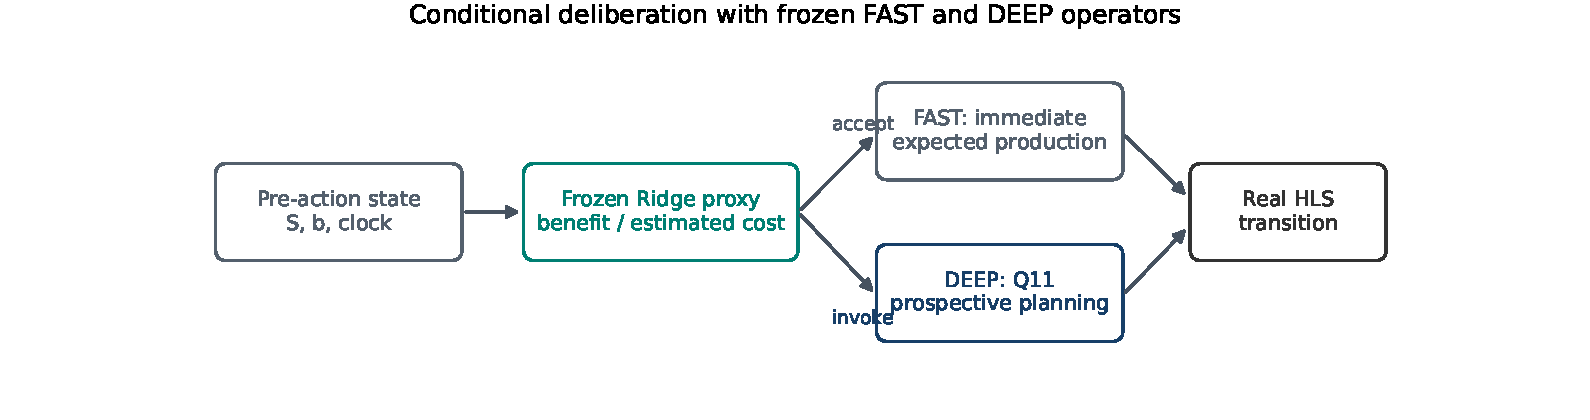
\includegraphics[width=.82\linewidth]{../../../results/campaigns/campaign3_meta_voc_confirmatory/analysis/figure1_architecture.pdf}\caption{Frozen conditional-deliberation routing architecture. The figure documents the evaluated system and is not a claim of algorithmic novelty.}\label{fig:architecture}\end{figure}
\begin{figure}[ht]\centering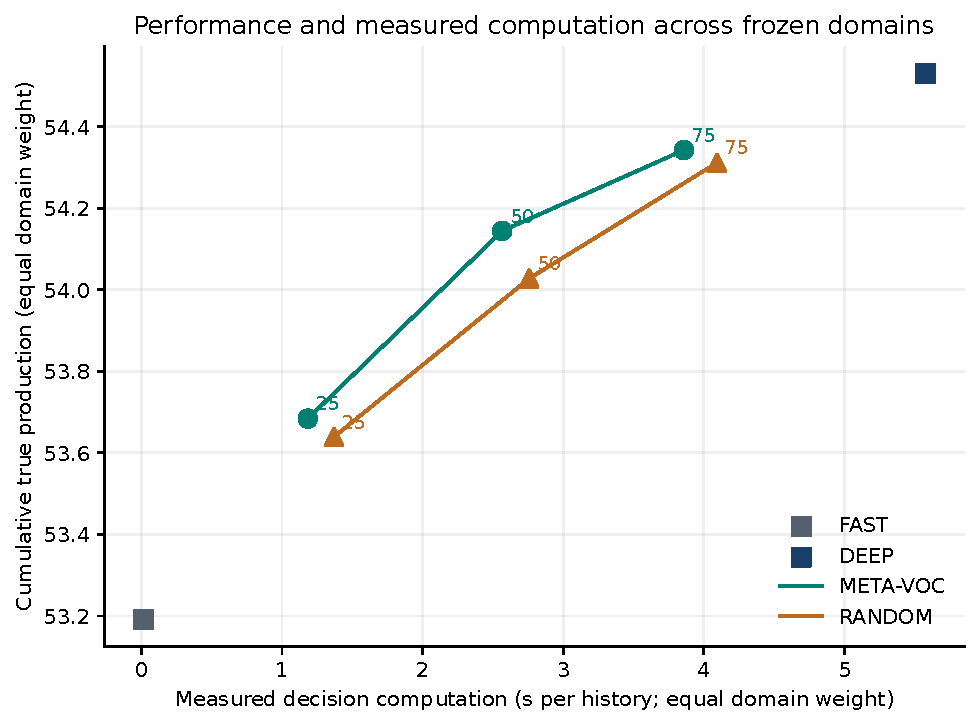
\includegraphics[width=.9\linewidth]{../../../results/campaigns/campaign3_meta_voc_confirmatory/analysis/figure2_performance_cost.pdf}\caption{Cumulative production against measured decision-computation time for the frozen confirmatory policies.}\label{fig:performance-cost}\end{figure}
\begin{figure}[ht]\centering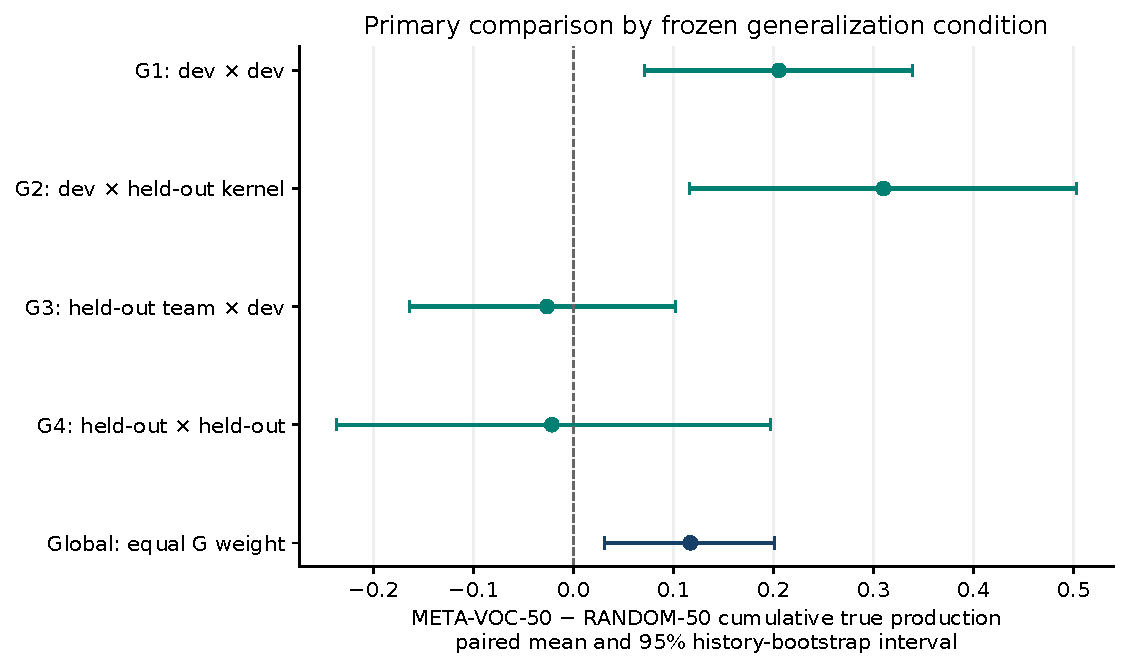
\includegraphics[width=.9\linewidth]{../../../results/campaigns/campaign3_meta_voc_confirmatory/analysis/figure3_primary_domain_effects.pdf}\caption{Paired META-VOC-50 minus RANDOM-50 production contrasts by frozen domain. Intervals crossing zero are not evidence of inferiority or equivalence.}\label{fig:domain-effects}\end{figure}
\begin{figure}[ht]\centering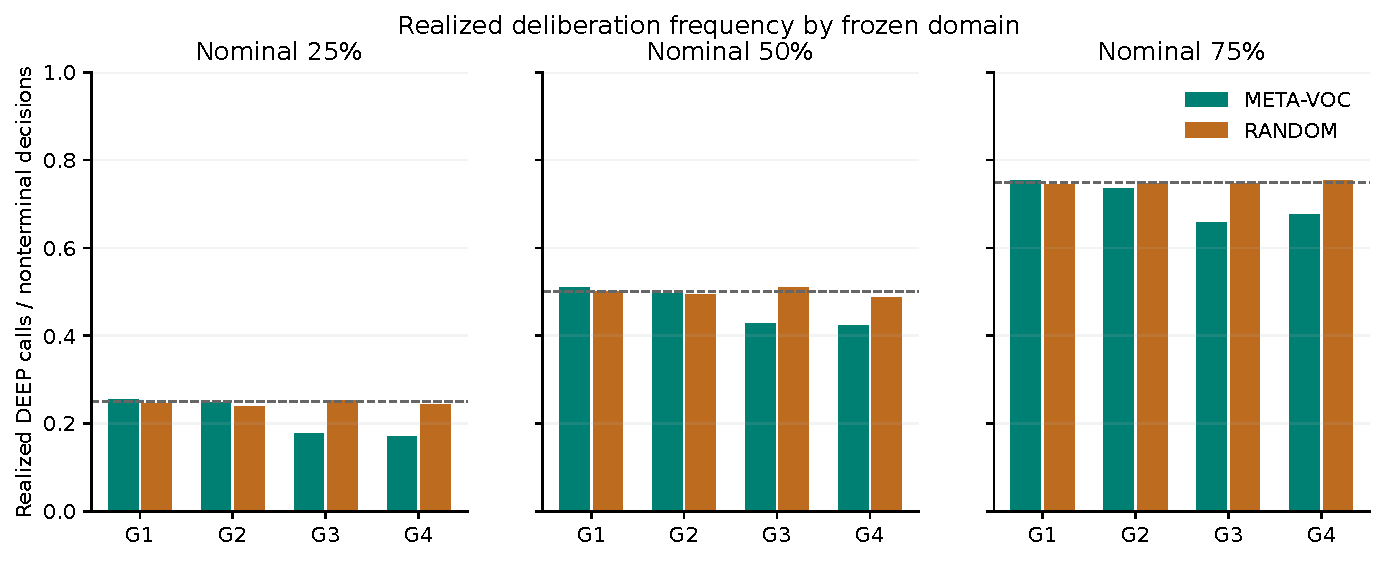
\includegraphics[width=.9\linewidth]{../../../results/campaigns/campaign3_meta_voc_confirmatory/analysis/figure4_invocation_rates.pdf}\caption{Realized DEEP invocation frequencies by domain and operating point.}\label{fig:invocation-rates}\end{figure}

\section{Conclusions}
A fixed state-informed conditional deliberation rule yielded a favorable but small equal-domain production--computation contrast relative to independent random invocation in a synthetic sequential team simulator. The production advantage was not established on held-out team geometries, and realized invocation budgets were unequal. These findings characterize one practical routing policy and its limits; they do not demonstrate a novel metareasoning principle, optimal computation allocation, or generalization to real organizations. The strongest scientific interpretation is a bounded empirical account of conditional prospective computation under evolving capabilities.

\bibliographystyle{plainnat}
\bibliography{references}
\end{document}
